\documentclass{article}
\usepackage{caption}
\usepackage{subcaption}
\usepackage{graphicx}

\title{CS 6073 Homework 2: Convolutional Neural Network}
\author{
    Luginbuhl, Dale \\
    \texttt{luginbdr@mail.uc.edu}
}
\date{September 30th 2023}


\begin{document}

\maketitle

\section{Data}
\subsection{How many data samples are included in the dataset?}
There are 70,000 samples included in the dataset. There are ten possible classses 
for the label, one corresponding to each digit. The total data set has 7,000 samples 
for each class.

\subsection{Which problem will this dataset try to address?}
The goal is to classify an image of a handwritten digit into one of ten classes.
The classes correspond to the integers in the range $[0,9]$.

\subsection{What is the minimum value and the maximum value in the dataset?}
The the input of each samlple is a single-channel monochrome image. The pixel values
are in the range $[0,255]$. The labels are in the range $[0,9]$.

\subsection{What is the dimension of each data sample?}
Each data sample is a 28x28 pixel monochrome image with a single channel. Each data 
sample therefore has 784 dimensions.

(i.e., pixels don't simply have a value of black and white, but a level of greyness from 0 to 255) as a result of the anti-aliasing technique used by the normalization algorithm

\subsection{Does the dataset have any missing information? E.g., missing features.}
The dataset does not have any missing information.

\subsection{What is the label of this dataset?}
The label of the dataset is an integer in the range $[0,9]$ representing the drawn 
digit.

\subsection{How many percent of data will you use for training, validation and testing?}
The dataset is pre-split into 60,000 training samples and 10,000 testing samples. All 
of the samples in the test set were drawn by different indivduals than the training 
set. There are 6,000 samples per class in the training set, and 1,000 samples per 
class in the training set.

We will further split the training set into a training set and a validation set.
The training set will consist of 50,000 samples and the validation set will consist
of 10,000 samples.

The resulting percentage splits will then be:
\begin{itemize}
    \item Training : 71.4\%
    \item Validation : 14.3\%
    \item Test : 14.3\%
\end{itemize}


\subsection{What kind of data pre-processing will you use for your training dataset?}
For each data sample, we will normalize the input, and one-hot encode the label.


\section{Model}
We will experiment with three different models. First a multilayer perceptron with 2 hidden
layers of width 32 and 16, and an output layer of width 10 (dnn). Second we implement
LeNet-5 (lenet). Third we consider ResNet18 (resnet).

\begin{table}[h]
\begin{center}
\begin{tabular}{c|c}
    Model & Accuracy \\
    \hline
    dnn & 96.41 \\
    lenet & 99.13 \\
    resnet & 99.14
\end{tabular}
\end{center}
\caption{Accuracy of highest performing models}
\label{table:evaluation_matrix}
\end{table}

\section{Objective}
Cross-entropy.

\section{Optimization}
We chose the Adam optimizer to take advantage of momentum in our optimization.
Adam allows us to converge to an optimum value more quickly, and it allows
provides the potential to escape from local minima.

\section{Model Selection}

\begin{table}[h]
\begin{center}
\begin{tabular}{c|c|c|c|c}
    Model & LR: 0.1 & LR: 0.01 & LR: 0.001 & LR: 0.0001 \\
    \hline
    dnn & 9.81 \& 0.12 & 92.71 \& 1.00 & 96.41 \& 1.00 & 86.31 \& 0.81 \\
    lenet & 9.74 \& 0.06 & 88.06 \& 1.00 & 99.13 \& 1.00 & 97.86 \& 1.00 \\
    resnet & 9.80 \& 0.06 & 98.06 \& 1.00 & 99.11 \& 1.00 & 99.14 \& 1.00
\end{tabular}
\end{center}
\caption{Impact of learning rate selection on model accuracy and F1 scores}
\label{table:learning_rate_selection}
\end{table}

In all of our models we achieved the best training results with a learning rate of
0.001 or 0.0001. Learning rates of 0.1 and 0.01 were too large for the training to be
stable. For the dnn and lenet model the best results were achieved at a learning rate
of 0.001. A learning rate of 0.0001 had the potential for superior results, but due to
the small learning rate size, the training required too much time. For the resnet model
we achieved the best results with a learning rate of 0.0001. Our results indicate that
perhaps using a learning rate scheduler could have yielded superior results. It would
allow us to have the benefits of a small learning rate, especially towards the end of
training, but without requiring too much time to train.

We didn't have much issue with underfitting or overfitting in our models. If we needed
to combat overfitting we could apply regularization, dropout, or data augmentation.


\section{Model Performance}

The best dnn model was the model trained with a learning rate of 0.001. The best
lenet model was the model trained with a learning rate of 0.001. The best resnet model
was the model trained with a learning rate of 0.0001. The best model overall was
the resnet, although it edged out the lenet model by a very slim margin. With more
fine-tuning, perhaps one of the models would emerge as the clear winner.

\begin{figure}[h]
    \centering
    \includegraphics[width=1.0\textwidth]{dnn_0.001/train_val_loss.png}
    \caption{Training and validation loss for dnn model with a learning rate of 0.001}
    \label{fig:dnn_0.001_loss}
\end{figure}

\begin{figure}[h]
    \centering
    \includegraphics[width=1.0\textwidth]{dnn_0.001/train_val_metrics.png}
    \caption{Training and validation accuracy and F1 scores for dnn model with a learning rate of 0.001}
    \label{fig:dnn_0.001_metrics}
\end{figure}

\begin{figure}[h]
    \centering
    \includegraphics[width=1.0\textwidth]{lenet_0.001/train_val_loss.png}
    \caption{Training and validation loss for lenet model with a learning rate of 0.001}
    \label{fig:lenet_0.001_loss}
\end{figure}

\begin{figure}[h]
    \centering
    \includegraphics[width=1.0\textwidth]{lenet_0.001/train_val_metrics.png}
    \caption{Training and validation accuracy and F1 scores for lenet model with a learning rate of 0.001}
    \label{fig:lenet_0.001_metrics}
\end{figure}

\begin{figure}[h]
    \centering
    \includegraphics[width=1.0\textwidth]{resnet_0.0001/train_val_loss.png}
    \caption{Training and validation loss for resnet model with a learning rate of 0.0001}
    \label{fig:resnet_0.0001_loss}
\end{figure}

\begin{figure}[h]
    \centering
    \includegraphics[width=1.0\textwidth]{resnet_0.0001/train_val_metrics.png}
    \caption{Training and validation accuracy and F1 scores for resnet model with a learning rate of 0.0001}
    \label{fig:resnet_0.0001_metrics}
\end{figure}

\begin{figure}[h]
    \centering
    \includegraphics[width=1.0\textwidth]{dnn_0.001/roc_curve.png}
    \caption{Test ROC curve for dnn model with a learning rate of 0.001}
    \label{fig:dnn_0.001_roc}
\end{figure}

\begin{figure}[h]
    \centering
    \includegraphics[width=1.0\textwidth]{lenet_0.001/roc_curve.png}
    \caption{Test ROC curve for lenet model with a learning rate of 0.001}
    \label{fig:lenet_0.001_roc}
\end{figure}

\begin{figure}[h]
    \centering
    \includegraphics[width=1.0\textwidth]{lenet_0.001/layer1_feats.png}
    \caption{First layer features for lenet model with a learning rate of 0.001}
    \label{fig:lenet_0.001_layer1_feats}
\end{figure}

\begin{figure}[h]
    \centering
    \includegraphics[width=1.0\textwidth]{lenet_0.001/layer2_feats.png}
    \caption{Second layer features for lenet model with a learning rate of 0.001}
    \label{fig:lenet_0.001_layer2_feats}
\end{figure}

\begin{figure}[h]
    \centering
    \includegraphics[width=1.0\textwidth]{resnet_0.0001/roc_curve.png}
    \caption{Test ROC curve for resnet model with a learning rate of 0.0001}
    \label{fig:resnet_0.0001_roc}
\end{figure}

\begin{figure}[h]
    \centering
    \includegraphics[width=1.0\textwidth]{resnet_0.0001/layer1_feats.png}
    \caption{First layer features for resnet model with a learning rate of 0.0001}
    \label{fig:resnet_0.0001_layer1_feats}
\end{figure}

\begin{figure}[h]
    \centering
    \includegraphics[width=1.0\textwidth]{resnet_0.0001/layer2_feats.png}
    \caption{Second layer features for resnet model with a learning rate of 0.0001}
    \label{fig:resnet_0.0001_layer2_feats}
\end{figure}

\end{document}